\documentclass[10pt,a4paper]{article}

\usepackage[utf8]{inputenc}		% Configuro la codificación
\input{.command.tex}
% En el siguiente archivo se configuran las variables del trabajo práctico
%% \providecommand es similar a \newcommnad, salvo que el primero ante un 
%% conflicto en la compilación, es ignorado.

% Al comienzo de un TP se debe modificar los argumentos de los comandos


\providecommand{\myTitle}{TRABAJO PRÁCTICO Nº2}
\providecommand{\mySubtitle}{Radiación}

\providecommand{\mySubject}{Electromagnestismo (82.06)}
\providecommand{\myKeywords}{UBA, Ingeniería, Informe, semiconductor}

\providecommand{\myAuthorSurname}{Alacaraz, Manso & Zuccolo}
\providecommand{\myTimePeriod}{Año 2018 - 1\textsuperscript{er} Cuatrimestre}

% No es necesario modificar este %%%%%%%%%%%%%%
\providecommand{\myHeaderLogo}{header_fiuba}
%%%%%%%%%%%%%%%%%%%%%%%%%%%%%%%%%%%%%%%%%%%%%%%%

% Si se utilizan listings, definir el lenguaje aquí
\providecommand{\myLanguage}{matlab}

% Crear los integrantes del TP con el comando \PutMember donde
%%		1) Apellido, Nombre
%%		2) Número de Padrón
%%		3) E-Mail
\providecommand{\MembersOnCover}[0]
{		\PutMember{Alcaraz, Gonzalo} {93874} {g.alcaraz@outlook.com}
		\PutMember{Manso, Juan} {96133} {juanmanso@gmail.com}
		\PutMember{Zuccolo, Florencia} {96628} {florenciaz618@gmail.com}
}

\providecommand{\myGroupNumber}{16}

\Pagebreaktrue		% Setea si hay un salto de página en la carátula
\Indextrue
\Siunitxtrue			% Si quiero utilizar el paquete, \siunixtrue. Si no \siunixfalse
\Todonotestrue		% Habilita/Deshabilita las To-Do Notes y las funciones \unsure, \change, \info, \improvement y \thiswillnotshow.
\Listingsfalse
\Keywordsfalse
\Putgrouptrue		% Habilita/Deshabilita el \myGroup en los headers
\Videofalse
				% Archivo con los comandos globales como Título y autores
\input{preamble.tex}

% Defino el path de los includegraphics
\graphicspath{{./Figuras/}{./imagenes/}}		% Directorio que contiene los graficos

% Defino el path para los input de .tex y de .eps
\makeatletter
\def\input@path{{./Figuras/}{./Secciones/}{./Cover_page/}{./imagenes}{./Tikz}}
\makeatother

% Defino el path del listings
\ifListings
%% Cambiar el nombre de la carpeta si se utilizan Listings
	\lstinputpath{../Secciones}
\fi


\begin{document}
		% Carátula (formal o simple,_formal o _simple respectivamente),
		% Resumen e Índice (si es necesario configurar en config.tex) del informe
		\input{cover_formal.tex}
	\setcounter{page}{1}
	\section{Desarrollo}
		\input{desarrollo.tex}
		\subsection{Método de momentos}
			\begin{equation}
	\centering
	V_m = \sum_{n=1}^N Z_{nm} I_m
\end{equation}

\begin{equation}
	\centering
	V_m = -j\omega \epsilon \int_{C(\bold{r})} E^i (\bold{r}) f_m(\bold{r}) d\bold{r}
\end{equation}	

\begin{equation}
	\centering
	Z_{nm} = \int_{C(\bold{r})} \int_{C(\bold{r'})} f_n(\bold{r'})\left[ \left(\frac{\partial^2}{\partial{z^2}} + \beta ^2 \right) G(\bold{r},\bold{r'}) \right] f_m(\bold{r}) d\bold{r'} d\bold{r}
\end{equation}


El método de momentos de la radiación se basa en la implementación de la ecuación de Pocklington. Para analizar la radiación de antenas, se divide la estructura metálica en elementos radiantes. Uno de estos elementos se conecta a una fuente de energía que se modela como fuente de tensión concentrada $V_m$. A partir de la resolución de un sistema lineal se obtiene la corriente de cada elemento que compone la estructura para una determinada frecuencia. Una vez obtenida la ditribución de corriente, se calcula el potencial vectorial \eqref{ec.A} y los campos eléctricos \eqref{ec.E} y magnéticos \eqref{ec.E} raidados por la estructura.

El software \textit{4nec2} permite resolver numéricamente las ecuaciones que describen la forma de la distribución de corriente ya sea proveniente de una fuente ó por inducción.

\begin{equation}
	\centering
	\bold{A} = \frac{\mu}{4 \cdot \pi} \int_{C(\bold{r'})} I(\bold{r'}) \frac{ \exp{(-i\beta R)} }{R} \bold{\hat{I}} dl'
	\label{ec.A}
\end{equation}	

\begin{equation}
	\centering
	\bold{E} = \frac{\nabla \times \bold{H} }{ j\omega\epsilon}
	\label{ec.E}
\end{equation}	

\begin{equation}
	\centering
	\bold{H} = \frac{\nabla \times \bold{H}}{j\omega \epsilon}
	\label{ec.H}
\end{equation}

	
		\subsection{Geometría a simular}
			\begin{figure}[H]
	\centering
	\scalebox{0.7}{% XCircuit output "config6.tex" for LaTeX input from config6.ps
\def\putbox#1#2#3#4{\makebox[0in][l]{\makebox[#1][l]{}\raisebox{\baselineskip}[0in][0in]{\raisebox{#2}[0in][0in]{\scalebox{#3}{#4}}}}}
\def\rightbox#1{\makebox[0in][r]{#1}}
\def\centbox#1{\makebox[0in]{#1}}
\def\topbox#1{\raisebox{-0.60\baselineskip}[0in][0in]{#1}}
\def\midbox#1{\raisebox{-0.20\baselineskip}[0in][0in]{#1}}
   \scalebox{1}{
   \normalsize
   \parbox{6.91667in}{
   \includegraphics[scale=1]{config6}\\
   % translate x=548 y=272 scale 0.38
   \putbox{3.2in}{0.08in}{1.20}{$\lambda$}%
   \putbox{4.99in}{0.06in}{1.20}{$\lambda/2$}%
   \putbox{2.04in}{0.97in}{1.20}{$\lambda/2$}%
   \putbox{1.22in}{0.08in}{1.20}{$\lambda/2$}%
   \putbox{6.1in}{0.08in}{1.20}{$\lambda/4$}%
   \putbox{0.66in}{0.97in}{1.20}{$\lambda/4$}%
   \putbox{5.5in}{0.95in}{1.20}{$\lambda/4$}%
   \putbox{0.06in}{0.08in}{1.20}{$\lambda/4$}%
   \putbox{4in}{0.95in}{1.20}{$\lambda/2$}%
   } % close 'parbox'
   } % close 'scalebox'
   \vspace{-\baselineskip} % this is not necessary, but looks better
}
	\caption{Configuración 6 asignada en dirección $z$.}
\end{figure}	




\begin{figure}[H]
	\begin{subfigure}{0.5\textwidth}
		\scalebox{0.7}{% XCircuit output "config6xy.tex" for LaTeX input from config6xy.ps
\def\putbox#1#2#3#4{\makebox[0in][l]{\makebox[#1][l]{}\raisebox{\baselineskip}[0in][0in]{\raisebox{#2}[0in][0in]{\scalebox{#3}{#4}}}}}
\def\rightbox#1{\makebox[0in][r]{#1}}
\def\centbox#1{\makebox[0in]{#1}}
\def\topbox#1{\raisebox{-0.60\baselineskip}[0in][0in]{#1}}
\def\midbox#1{\raisebox{-0.20\baselineskip}[0in][0in]{#1}}
   \scalebox{1}{
   \normalsize
   \parbox{4.1875in}{
   \includegraphics[scale=1]{config6xy}\\
   % translate x=540 y=424 scale 0.38
   \putbox{1.85in}{0.7in}{1.20}{\rotatebox{-270}{\tiny{$\lambda = \SI{3.75}{\meter}$}}}%
   \putbox{0.85in}{0.7in}{1.20}{\rotatebox{-270}{\tiny{$\lambda /2 = \SI{1.875}{\meter}$}}}%
   \putbox{0.35in}{0.7in}{1.20}{\rotatebox{-270}{\tiny{$\lambda /4 = \SI{0.9375}{\meter}$}}}%
   \putbox{2.85in}{0.7in}{1.20}{\rotatebox{-270}{\tiny{$\lambda /2 = \SI{1.875}{\meter}$}}}%
   \putbox{3.4in}{0.7in}{1.20}{\rotatebox{-270}{\tiny{$\lambda /4 = \SI{0.9375}{\meter}$}}}%
   \putbox{2.14in}{2.89in}{1.20}{$z$}%
   \putbox{4.14in}{0.56in}{1.20}{$x$}%
   \putbox{1.2in}{0.26in}{1.20}{{\tiny{$\lambda /2 = \SI{1.875}{\meter}$}}}%
   \putbox{2.2in}{0.26in}{1.20}{{\tiny{$\lambda /2 = \SI{1.875}{\meter}$}}}%
   \putbox{0.58in}{0.26in}{1.20}{\tiny{$\lambda /4=$}}%
   \putbox{3.18in}{0.26in}{1.20}{\tiny{$\lambda /4=$}}%
   \putbox{0.5in}{0.15in}{1.20}{\tiny{$\SI{0.9375}{\meter}$}}%
   \putbox{3.1in}{0.15in}{1.20}{\tiny{$\SI{0.9375}{\meter}$}}%
   } % close 'parbox'
   } % close 'scalebox'
   \vspace{-\baselineskip} % this is not necessary, but looks better
}
		\caption{Configuración 6 asignada (plano $xz$).}
		\label{fig.config_xz}
	\end{subfigure}
	\quad
	\begin{subfigure}{0.5\textwidth}
		\includegraphics[scale=0.4]{imagenes/2_geometria.png}
		\caption{Geometría ingresada en el programa \textit{4nec2}.}
	\end{subfigure}
\end{figure}

%\begin{figure}[H]
%	\centering
%	\scalebox{0.9}{% XCircuit output "config6xy.tex" for LaTeX input from config6xy.ps
\def\putbox#1#2#3#4{\makebox[0in][l]{\makebox[#1][l]{}\raisebox{\baselineskip}[0in][0in]{\raisebox{#2}[0in][0in]{\scalebox{#3}{#4}}}}}
\def\rightbox#1{\makebox[0in][r]{#1}}
\def\centbox#1{\makebox[0in]{#1}}
\def\topbox#1{\raisebox{-0.60\baselineskip}[0in][0in]{#1}}
\def\midbox#1{\raisebox{-0.20\baselineskip}[0in][0in]{#1}}
   \scalebox{1}{
   \normalsize
   \parbox{4.1875in}{
   \includegraphics[scale=1]{config6xy}\\
   % translate x=540 y=424 scale 0.38
   \putbox{1.85in}{0.7in}{1.20}{\rotatebox{-270}{\tiny{$\lambda = \SI{3.75}{\meter}$}}}%
   \putbox{0.85in}{0.7in}{1.20}{\rotatebox{-270}{\tiny{$\lambda /2 = \SI{1.875}{\meter}$}}}%
   \putbox{0.35in}{0.7in}{1.20}{\rotatebox{-270}{\tiny{$\lambda /4 = \SI{0.9375}{\meter}$}}}%
   \putbox{2.85in}{0.7in}{1.20}{\rotatebox{-270}{\tiny{$\lambda /2 = \SI{1.875}{\meter}$}}}%
   \putbox{3.4in}{0.7in}{1.20}{\rotatebox{-270}{\tiny{$\lambda /4 = \SI{0.9375}{\meter}$}}}%
   \putbox{2.14in}{2.89in}{1.20}{$z$}%
   \putbox{4.14in}{0.56in}{1.20}{$x$}%
   \putbox{1.2in}{0.26in}{1.20}{{\tiny{$\lambda /2 = \SI{1.875}{\meter}$}}}%
   \putbox{2.2in}{0.26in}{1.20}{{\tiny{$\lambda /2 = \SI{1.875}{\meter}$}}}%
   \putbox{0.58in}{0.26in}{1.20}{\tiny{$\lambda /4=$}}%
   \putbox{3.18in}{0.26in}{1.20}{\tiny{$\lambda /4=$}}%
   \putbox{0.5in}{0.15in}{1.20}{\tiny{$\SI{0.9375}{\meter}$}}%
   \putbox{3.1in}{0.15in}{1.20}{\tiny{$\SI{0.9375}{\meter}$}}%
   } % close 'parbox'
   } % close 'scalebox'
   \vspace{-\baselineskip} % this is not necessary, but looks better
}
%	\caption{Configuración 6 asignada (plano $xz$).}
%\end{figure}

%\begin{figure}[H]
%	\centering
%	\includegraphics[scale=0.5]{imagenes/2_geometria.png}
%	\caption{Geometría ingresada en el programa \textit{4nec2}.}
%\end{figure}
		\subsection{Diagramas de radiación}
			\begin{figure}[H]
	\begin{subfigure}{0.5\textwidth}
		\includegraphics[scale=0.43]{imagenes/2D_80MHz.png}
	\end{subfigure}	
	\quad
	\begin{subfigure}{0.5\textwidth}
		\includegraphics[scale=0.43]{imagenes/3D_80MHz.png}
	\end{subfigure}
	\caption{$f=\SI{80}{\mega\hertz}$}
	\label{fig.radiacion_80M}
\end{figure}


\begin{figure}[H]
	\begin{subfigure}{0.5\textwidth}
		\includegraphics[scale=0.43]{imagenes/2D_160MHz.png}
	\end{subfigure}	
	\quad
	\begin{subfigure}{0.5\textwidth}
		\includegraphics[scale=0.43]{imagenes/3D_160MHz.png}
	\end{subfigure}
	\caption{$f=\SI{160}{\mega\hertz}$}
	\label{fig.radiacion_160M}
\end{figure}


\begin{figure}[H]
	\begin{subfigure}{0.5\textwidth}
		\includegraphics[scale=0.43]{imagenes/2D_240MHz.png}
	\end{subfigure}	
	\quad
	\begin{subfigure}{0.5\textwidth}
		\includegraphics[scale=0.43]{imagenes/3D_240MHz.png}
	\end{subfigure}
	\caption{$f=\SI{240}{\mega\hertz}$}
	\label{fig.radiacion_240M}
\end{figure}


\begin{figure}[H]
	\begin{subfigure}{0.5\textwidth}
		\includegraphics[scale=0.43]{imagenes/2D_320MHz.png}
	\end{subfigure}	
	\quad
	\begin{subfigure}{0.5\textwidth}
		\includegraphics[scale=0.43]{imagenes/3D_320MHz.png}
	\end{subfigure}
	\caption{$f=\SI{320}{\mega\hertz}$.}
	\label{fig.radiacion_320M}
\end{figure}


\begin{figure}[H]
	\begin{subfigure}{0.5\textwidth}
		\includegraphics[scale=0.43]{imagenes/2D_400MHz.png}
	\end{subfigure}	
	\quad
	\begin{subfigure}{0.5\textwidth}
		\includegraphics[scale=0.43]{imagenes/3D_400MHz.png}
	\end{subfigure}
	\caption{$f=\SI{400}{\mega\hertz}$.}
	\label{fig.radiacion_400M}
\end{figure}



\begin{figure}[H]
	\begin{subfigure}{0.5\textwidth}
		\includegraphics[scale=0.43]{imagenes/2D_480MHz.png}
	\end{subfigure}	
	\quad
	\begin{subfigure}{0.5\textwidth}
		\includegraphics[scale=0.43]{imagenes/3D_480MHz.png}
	\end{subfigure}
	\caption{$f=\SI{480}{\mega\hertz}$.}
	\label{fig.radiacion_480M}
\end{figure}	

		\subsection{Gráfico de corriente}
			\begin{figure}[H]
	\begin{subfigure}{0.5\textwidth}
		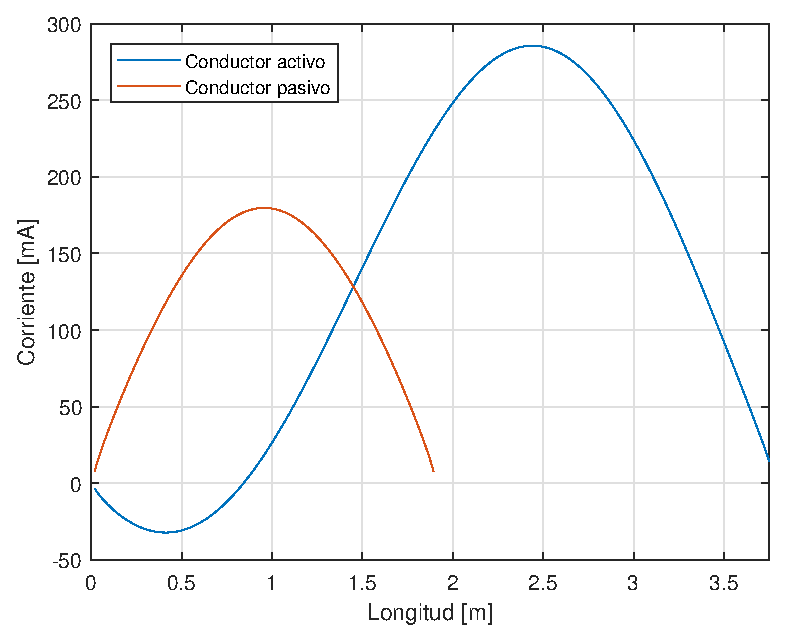
\includegraphics[scale=0.6]{imagenes/i_real_80.eps}
		\caption{Parte real.}
		\label{fig.i_real_80}
	\end{subfigure}
	\quad
	\begin{subfigure}{0.5\textwidth}
		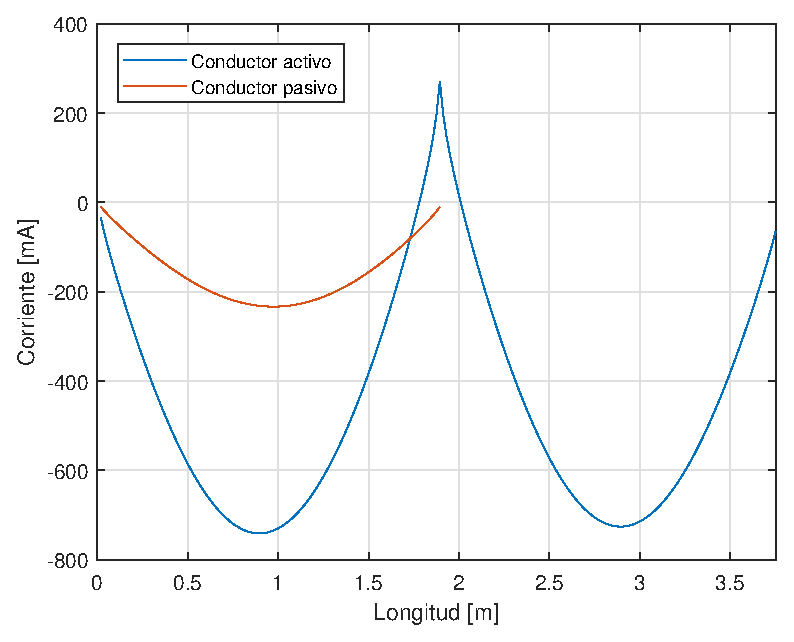
\includegraphics[scale=0.6]{imagenes/i_imag_80.eps}
		\caption{Parte imaginaria.}
		\label{fig.i_imag_80}
	\end{subfigure}
	\quad
	\begin{subfigure}{0.5\textwidth}
		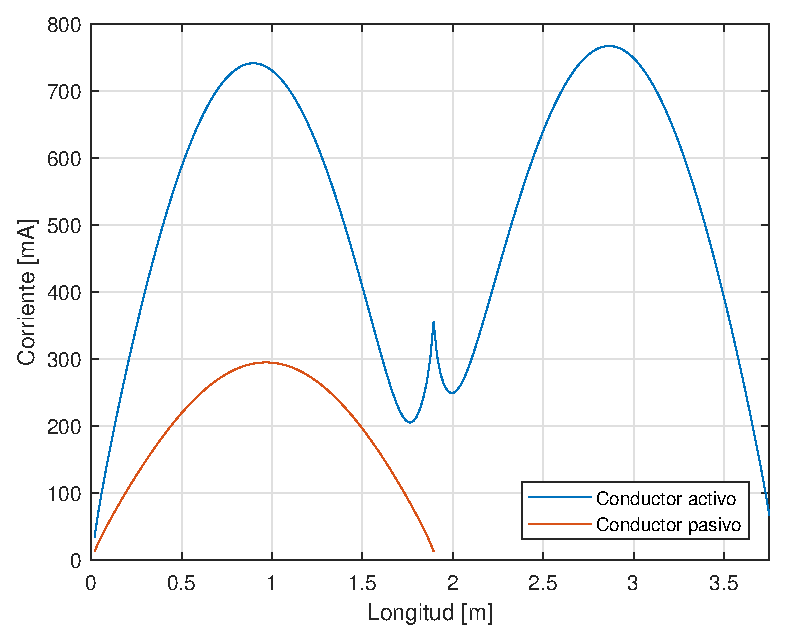
\includegraphics[scale=0.6]{imagenes/i_mag_80.eps}
		\caption{Magnitud.}
		\label{fig.i_mag_80}		
	\end{subfigure}
	\quad
	\begin{subfigure}{0.5\textwidth}
		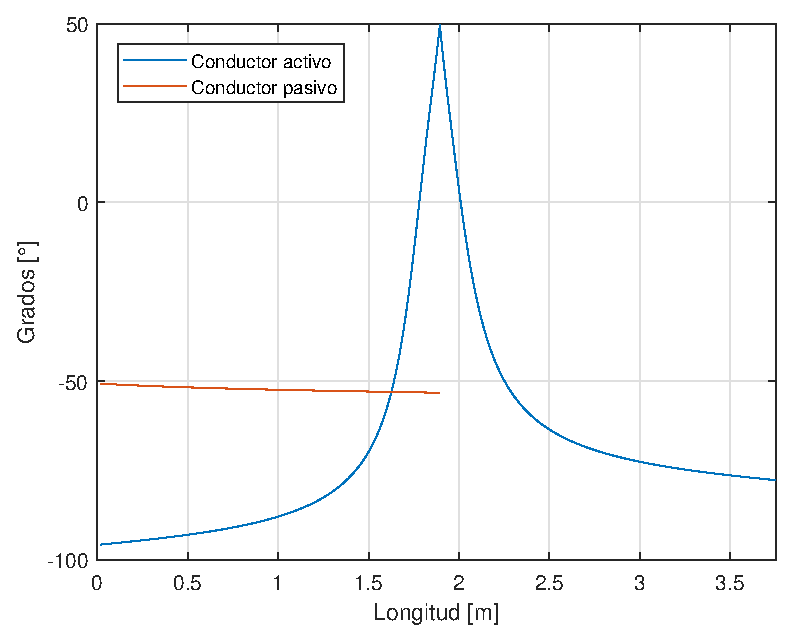
\includegraphics[scale=0.6]{imagenes/i_fase_80.eps}
		\caption{Fase.}
		\label{fig.i_fase_80}		
	\end{subfigure}
	\caption{Corriente para la frecuencia mínima $f = \SI{80}{\mega\hertz}$}
	\label{fig.i_80}	
\end{figure}

En las figuras \ref{fig.i_80} se muestra la corriente para $f=\SI{80}{\mega\hertz}$ en el conductor activo y en uno de los conductores pasivos. Se eligió el que se encuentra a la derecha del mismo a una distancia de $\lambda/2$. Como era de esperarse, la magnitud de la corriente es mayor en el conductor activo que en el pasivo. La diferencia de magnitud de las corrientes máximas entre ambos conductores es de aproximadamente $\SI{440}{\milli\ampere}$. La fase del conductor pasivo se mantiene prácticamente constante, mientras que en conductor activo cambia drásticamente en la mitad de la longitud del mismo ($\SI{1.9}{\meter}$) y luego tiende a acercarse a su valor inicial.

\begin{figure}[H]
	\begin{subfigure}{0.5\textwidth}
		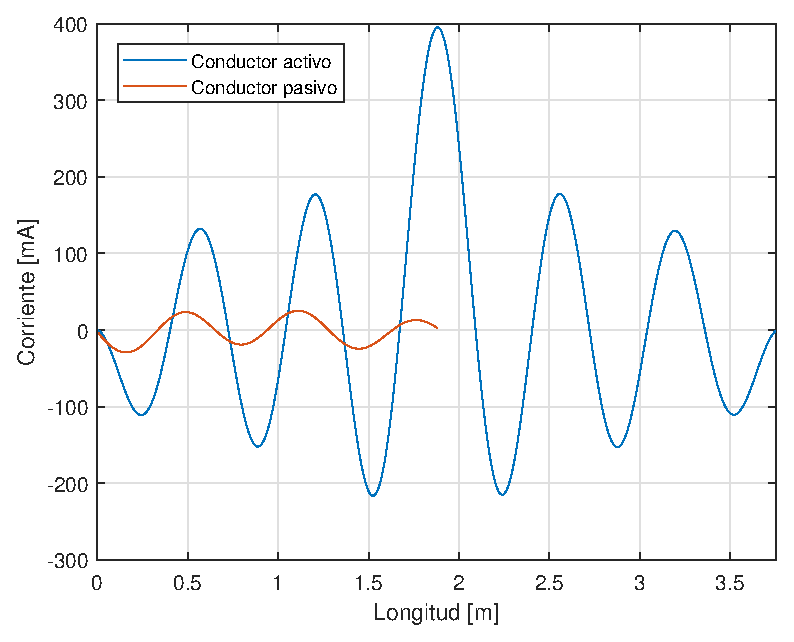
\includegraphics[scale=0.6]{imagenes/i_real_480.eps}
		\caption{Parte real.}
		\label{fig.i_real_480}	
	\end{subfigure}
	\quad
	\begin{subfigure}{0.5\textwidth}
		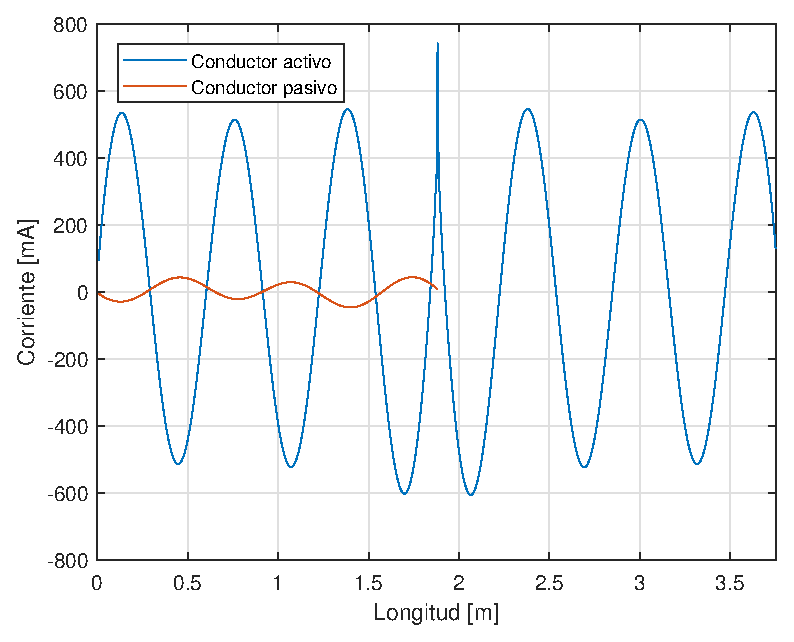
\includegraphics[scale=0.6]{imagenes/i_imag_480.eps}
		\caption{Parte imaginaria.}
		\label{fig.i_imag_480}
	\end{subfigure}
	\quad
	\begin{subfigure}{0.5\textwidth}
		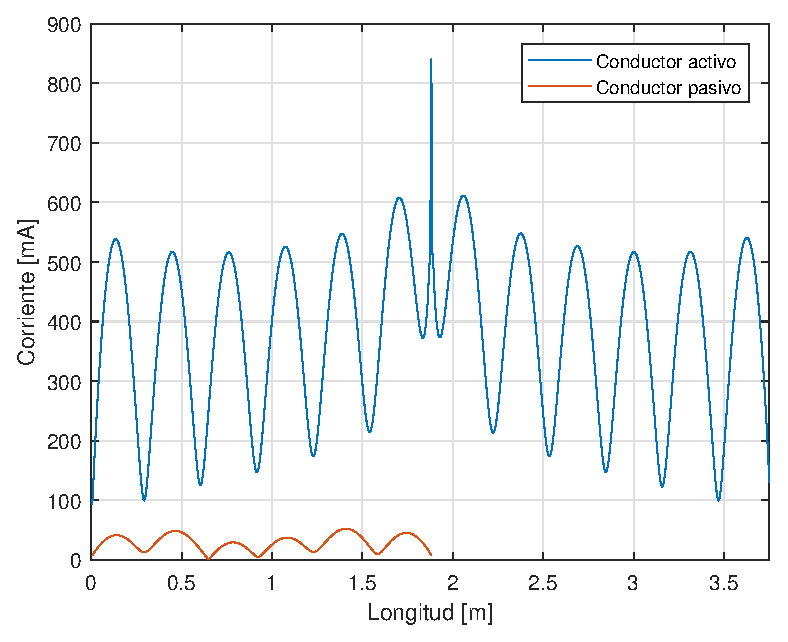
\includegraphics[scale=0.6]{imagenes/i_mag_480.eps}
		\caption{Magnitud.}
		\label{fig.i_mag_480}
	\end{subfigure}
	\quad
	\begin{subfigure}{0.5\textwidth}
		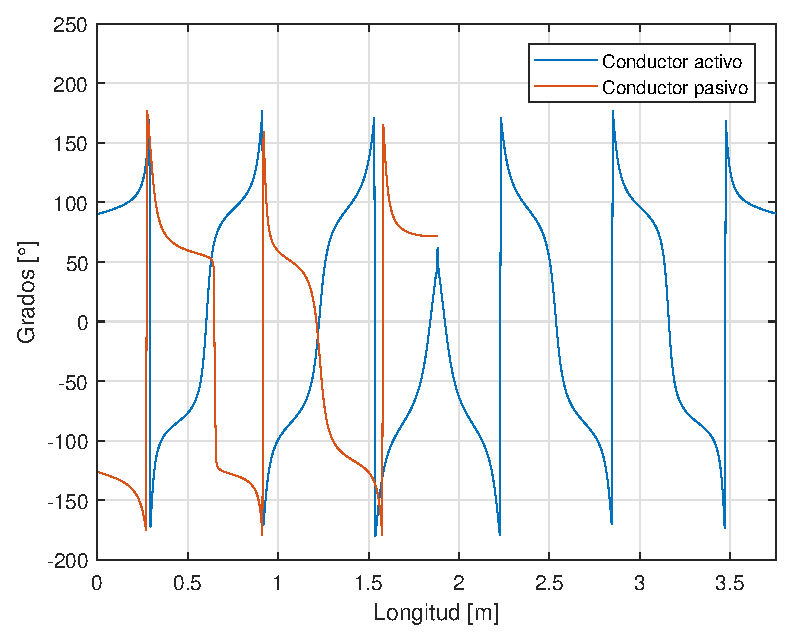
\includegraphics[scale=0.6]{imagenes/i_fase_480.eps}
		\caption{Fase.}
		\label{fig.i_fase_480}
	\end{subfigure}
	\caption{Corriente para la frecuencia máxima $f = \SI{480}{\mega\hertz}$}
	\label{fig.i_480}
\end{figure}


Análogamente se realizaron los gráficos para la máxima frecuencia. La diferencia de magnitud de las corrientes máximas entre ambos conductores es de $\SI{500}{\milli\ampere}$. Se observa que la corriente en el conductor pasivo se encuentra en contrafase al activo. Al comparar las figuras \ref{fig.i_mag_80} y \ref{fig.i_mag_480} se aprecia que entre $\SI{1.8}{\meter}$ y $\SI{2}{\meter}$, la magnitud de la corriente del conductor activo para $f=\SI{80}{\mega\hertz}$ es mínima, mientras que para $f=\SI{480}{\mega\hertz}$ es máxima.
		\subsection{Resistencia de radiación}
			\begin{figure}[H]
	\centering
	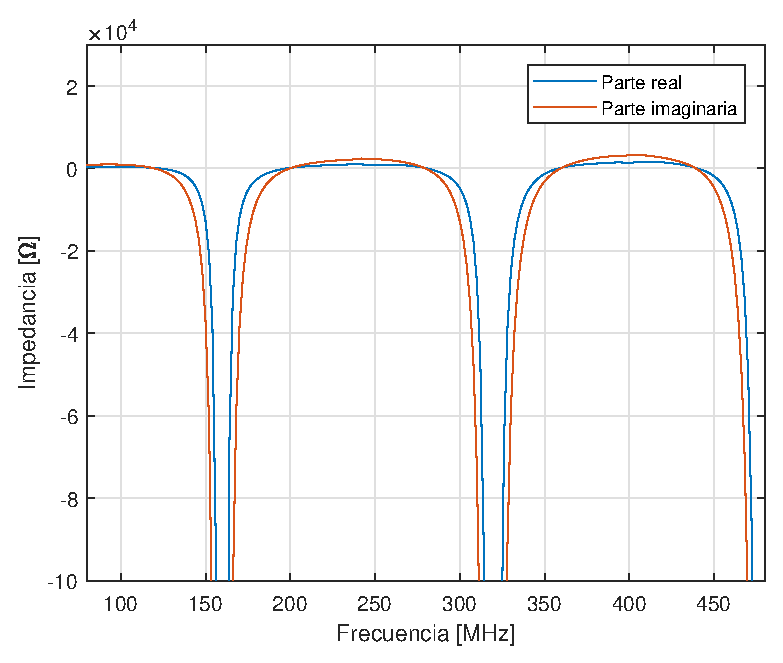
\includegraphics{imagenes/z.eps}
	\caption{Resistencia de radiación.}
	\label{fig.z_radiacion}
\end{figure}
		\subsection{Diseño de adaptador de impedancia}
			La adaptación permite obtener una máxima eficiencia en la transmisión de energía, eliminando reflexiones de onda. Dentro de las posibles formas de adaptación, se optó por la utilización del adaptador de cuarto de onda y stub. La línea opera en un entorno de la mínima frecuencia, $\SI{72}{\mega\hertz} < f < \SI{88}{\mega\hertz}$ (se realiza el \emph{sweep} cada \SI{1}{\mega\hertz}), por lo que se considera el valor de carga de la expresión \eqref{ec.z_80}.

A su vez se considera un criterio de $|\rho_l|<0,2$, o de forma equivalente $\rm{ROE} \leq 1,5$

\subsection{Adaptador de cuarto de onda}
El proceso consiste en intercalar el adaptador a una distancia $z_s$ de la carga $Z_L$, de forma tal que la impedancia de entrada $Z_{in}$ del conjunto línea y carga sea real. Para hallar el valor de $z_s$ se utiliza la carta de Smith mediante software. El adaptador queda definido mediante los parámetros $z_a$ (impedancia del adaptador) y $L_a$ (longitud del adaptador). La impedancia característica de la línea es dato, $Z_o = \SI{50}{\ohm}$. Ubicandose en $Z_L$, se desplaza hacia el generador sobre la circuinferencia $|\rho_L|$ hasta obtener impedancia real (eje real). Así se obtiene longitud de arco recorrido da la posición $z_s$ del adaptador. A partir de dicho valor y $Z_{in}$ se obtienen los parámetros de la línea \eqref{ec.z_a_4} y \eqref{ec.L_a_4}.

\begin{equation}
	\centering
	Z_a = \sqrt{Z_o \cdot Z_{in}} = \sqrt{ \SI{50}{\ohm} \cdot \SI{1.38}{\ohm} } = \SI{8.3}{\ohm}
	\label{ec.z_a_4}
\end{equation}	

\begin{equation}
	\centering
	L_a = \frac{\lambda_a}{4} = \frac{ \SI{3.75}{\meter} }{4} = \SI{0.937}{\meter}
	\label{ec.L_a_4}
\end{equation}


%%%% FIGURA PARA CUARTO DE ONDA ESPACIO LIBRE
\begin{figure}[H]
	\centering
	\includegraphics[scale=0.83]{imagenes/smith_4_espacio_libre_esq.png}
	\label{fig.smith_4_esq}
\end{figure}
\begin{figure}[H]
	\centering
	\includegraphics[scale=0.63]{imagenes/smith_4_espacio_libre.png}
	\label{fig.smith_4}
\end{figure}



\subsection{Stub}

La adaptación mediante \texttt{stub} consiste en anexar un trozo de la misma línea conectada en paralelo. Normalmente, para evitar interferencias se suele cortocircuitar el extremo de la carga. Se parte del punto de impedancia obtenido en \emph{4nec2} hasta llegar a la circunferencia de impedancia real unitaria moviéndose hacia el generador. Allí se coloca el stub cuyo largo será el necesario hasta llegar al centro de la carta recorriendo la circunferencia de impedancia real unitaria en sentido antihorario. Utilizando el programa se obtiene:

\begin{equation*}
	\centering
	L_s = \num{0.0269}\cdot \lambda = \SI{100.8}{\milli\m}
\end{equation*}

\begin{equation*}
	\centering
	d_s = \num{0.2195}\cdot \lambda = \SI{822.5}{\milli\m}
\end{equation*}


%%%% FIGURA PARA STUB ESPACIO LIBRE
\begin{figure}[H]
	\centering
	\includegraphics[scale=0.83]{imagenes/smith_stub_espacio_libre_esq.png}
	\label{fig.smith_stub_esq}
\end{figure}

\begin{figure}[H]
	\centering
	\includegraphics[scale=0.63]{imagenes/smith_stub_espacio_libre.png}
	\label{fig.smith_stub}
\end{figure}




		\subsection{Plano de tierra perfecto}
			%%%%%%%%%% 2. Geometría %%%%%%%%%%%%

\begin{figure}[H]
	\centering
	\includegraphics[scale=0.4]{imagenes/2_geometria_tierra.png}
	\caption{Geometría ingresada con plano a tierra perfecto.}
	\label{fig.geometria_tierra}
\end{figure}

%%%%%%%%%% 3. Diagramas de radiación %%%%%%%%%%

\begin{figure}[H]
	\begin{subfigure}{0.5\textwidth}
		\includegraphics[scale=0.43]{imagenes/2D_80MHz_tierra.png}
	\end{subfigure}	
	\quad
	\begin{subfigure}{0.5\textwidth}
		\includegraphics[scale=0.43]{imagenes/3D_80MHz_tierra.png}
	\end{subfigure}
	\caption{$f=\SI{80}{\mega\hertz}$}
	\label{fig.radiacion_80M_tierra}
\end{figure}


\begin{figure}[H]
	\begin{subfigure}{0.5\textwidth}
		\includegraphics[scale=0.43]{imagenes/2D_160MHz_tierra.png}
	\end{subfigure}	
	\quad
	\begin{subfigure}{0.5\textwidth}
		\includegraphics[scale=0.43]{imagenes/3D_160MHz_tierra.png}
	\end{subfigure}
	\caption{$f=\SI{160}{\mega\hertz}$}
	\label{fig.radiacion_160M_tierra}
\end{figure}


\begin{figure}[H]
	\begin{subfigure}{0.5\textwidth}
		\includegraphics[scale=0.43]{imagenes/2D_240MHz_tierra.png}
	\end{subfigure}	
	\quad
	\begin{subfigure}{0.5\textwidth}
		\includegraphics[scale=0.43]{imagenes/3D_240MHz_tierra.png}
	\end{subfigure}
	\caption{$f=\SI{240}{\mega\hertz}$}
	\label{fig.radiacion_240M_tierra}
\end{figure}


\begin{figure}[H]
	\begin{subfigure}{0.5\textwidth}
		\includegraphics[scale=0.43]{imagenes/2D_320MHz_tierra.png}
	\end{subfigure}	
	\quad
	\begin{subfigure}{0.5\textwidth}
		\includegraphics[scale=0.43]{imagenes/3D_320MHz_tierra.png}
	\end{subfigure}
	\caption{$f=\SI{320}{\mega\hertz}$.}
	\label{fig.radiacion_320M_tierra}
\end{figure}


\begin{figure}[H]
	\begin{subfigure}{0.5\textwidth}
		\includegraphics[scale=0.43]{imagenes/2D_400MHz_tierra.png}
	\end{subfigure}	
	\quad
	\begin{subfigure}{0.5\textwidth}
		\includegraphics[scale=0.43]{imagenes/3D_400MHz_tierra.png}
	\end{subfigure}
	\caption{$f=\SI{400}{\mega\hertz}$.}
	\label{fig.radiacion_400M_tierra}
\end{figure}



\begin{figure}[H]
	\begin{subfigure}{0.5\textwidth}
		\includegraphics[scale=0.43]{imagenes/2D_480MHz_tierra.png}
	\end{subfigure}	
	\quad
	\begin{subfigure}{0.5\textwidth}
		\includegraphics[scale=0.43]{imagenes/3D_480MHz_tierra.png}
	\end{subfigure}
	\caption{$f=\SI{480}{\mega\hertz}$.}
	\label{fig.radiacion_480M_tierra}
\end{figure}	

%%%%%%%%%% 4. CORRIENTES %%%%%%%%%%
\begin{figure}[H]
	\begin{subfigure}{0.5\textwidth}
		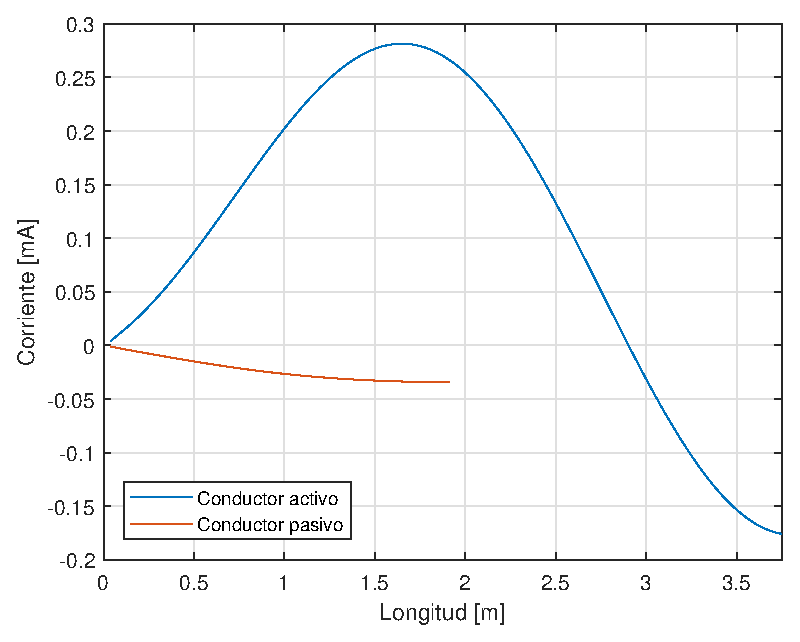
\includegraphics[scale=0.6]{imagenes/i_real_80_tierra.eps}
		\caption{Parte real.}
	\end{subfigure}
	\quad
	\begin{subfigure}{0.5\textwidth}
		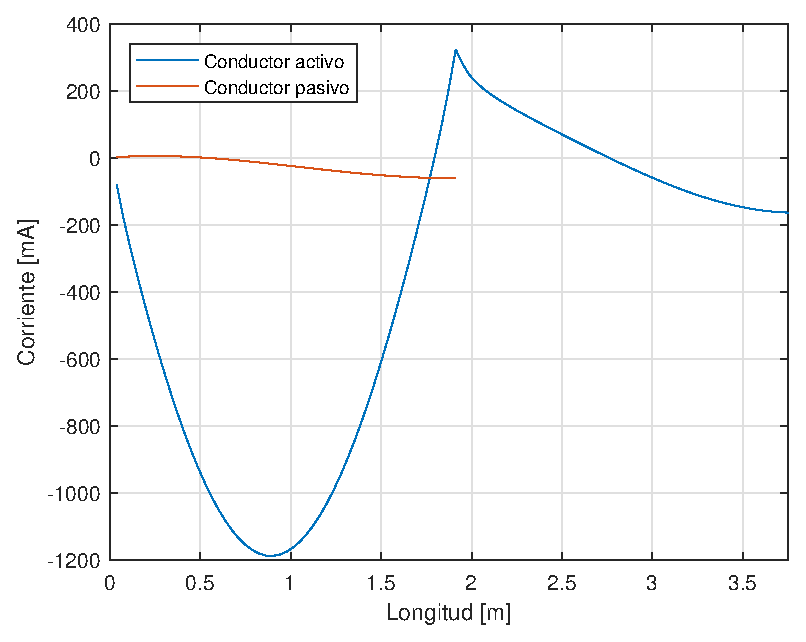
\includegraphics[scale=0.6]{imagenes/i_imag_80_tierra.eps}
		\caption{Parte imaginaria.}
	\end{subfigure}
	\quad
	\begin{subfigure}{0.5\textwidth}
		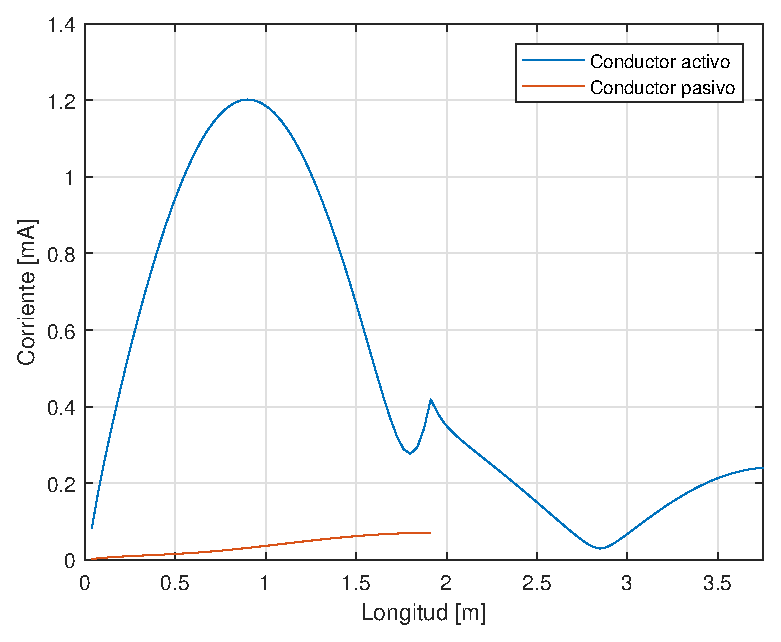
\includegraphics[scale=0.6]{imagenes/i_mag_80_tierra.eps}
		\caption{Magnitud.}
	\end{subfigure}
	\quad
	\begin{subfigure}{0.5\textwidth}
		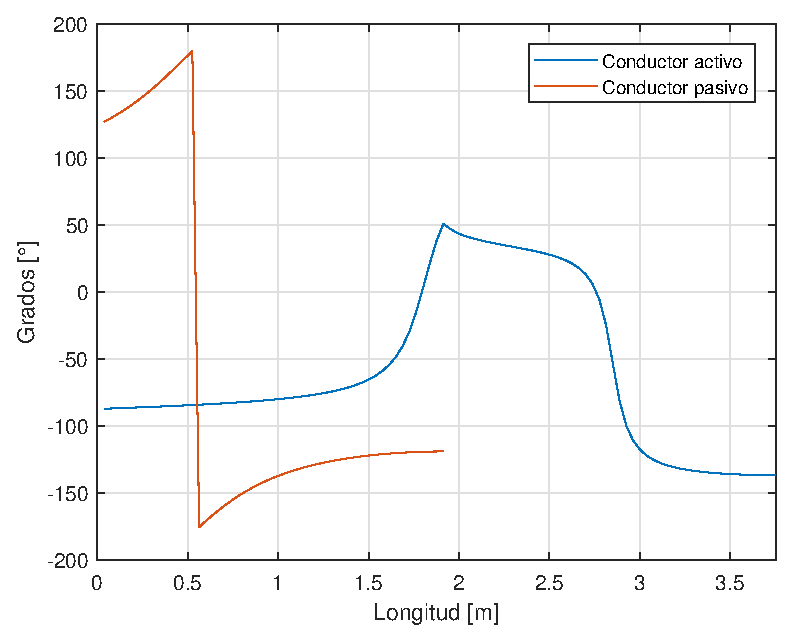
\includegraphics[scale=0.6]{imagenes/i_fase_80_tierra.eps}
		\caption{Fase.}
	\end{subfigure}
	\caption{Corriente para la frecuencia mínima $f = \SI{80}{\mega\hertz}$}
\end{figure}


\begin{figure}[H]
	\begin{subfigure}{0.5\textwidth}
		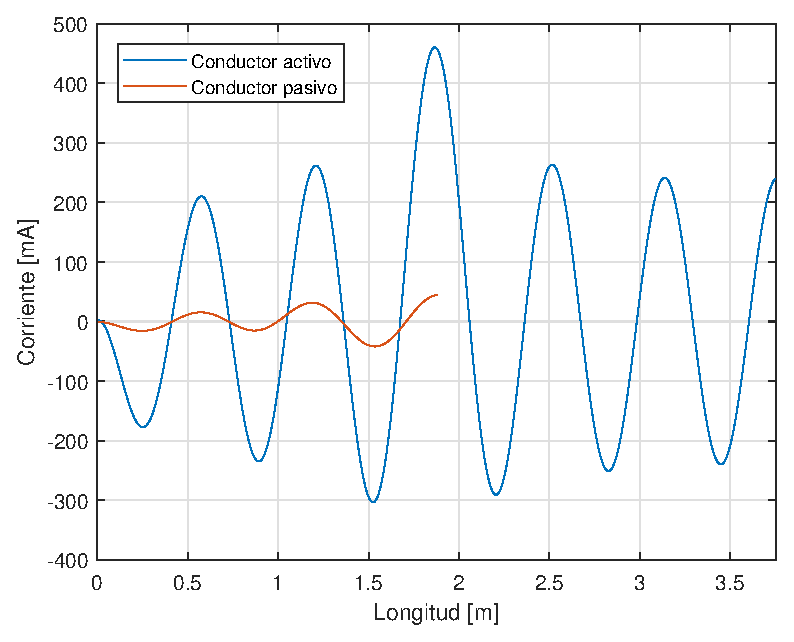
\includegraphics[scale=0.6]{imagenes/i_real_480_tierra.eps}
		\caption{Parte real.}
	\end{subfigure}
	\quad
	\begin{subfigure}{0.5\textwidth}
		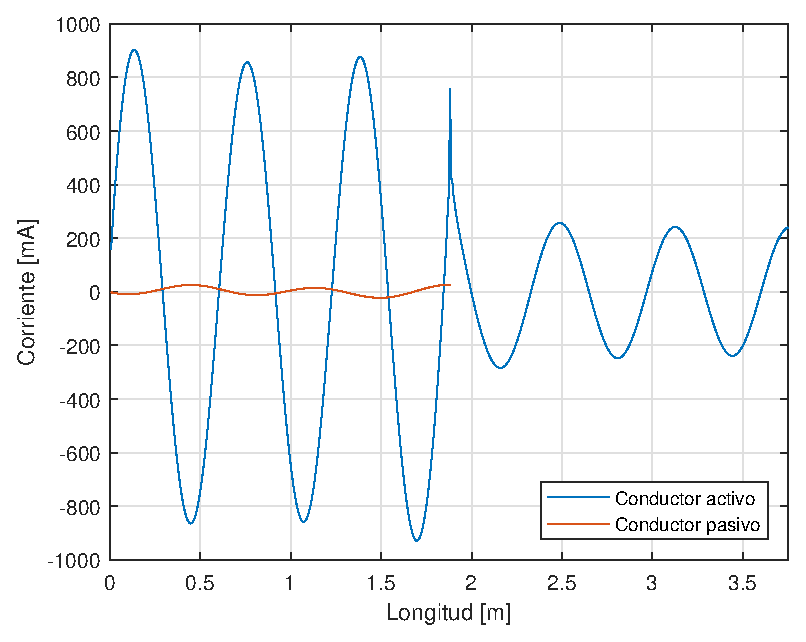
\includegraphics[scale=0.6]{imagenes/i_imag_480_tierra.eps}
		\caption{Parte imaginaria.}
	\end{subfigure}
	\quad
	\begin{subfigure}{0.5\textwidth}
		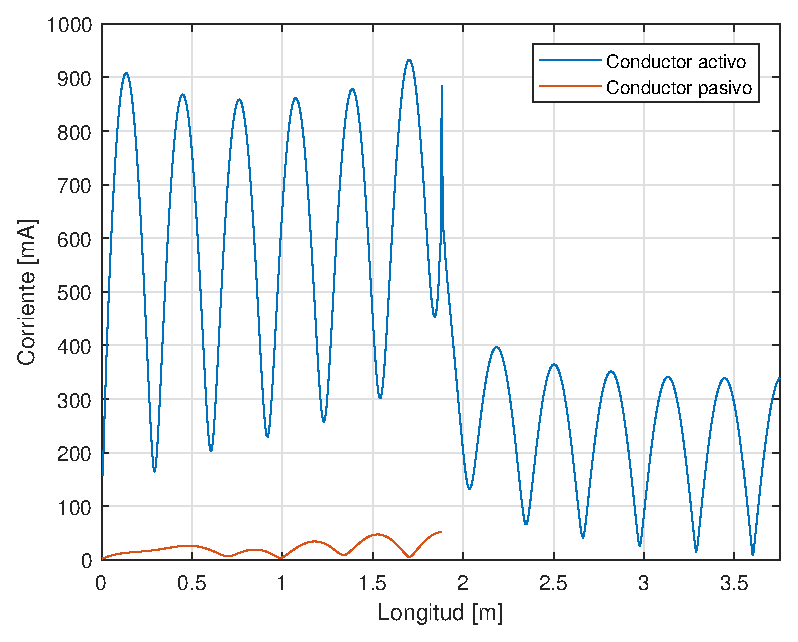
\includegraphics[scale=0.6]{imagenes/i_mag_480_tierra.eps}
		\caption{Magnitud.}
	\end{subfigure}
	\quad
	\begin{subfigure}{0.5\textwidth}
		\includegraphics[scale=0.6]{imagenes/i_fase_480_tierra.eps}
		\caption{Fase.}
	\end{subfigure}
	\caption{Corriente para la frecuencia máxima $f = \SI{480}{\mega\hertz}$}
\end{figure}		
	\pagebreak					
	\section{Conclusiones}
		En base a las simulaciones realizadas se logró determinar la radiación emitida por cierta configuración, resultando un correcto funcionamiento sólo para algunas frecuencias debido a la aparición de lóbulos secundarios capaces de desviar la directividad de la antena.
		
	%\appendix
\end{document}
